% snapguard_revision.tex — from snapguard_overleaf_10062026.tex
% Edits for reviewers: NEW text in \ben{...} (blue); OLD text kept as % comments.
% Tracker: snapguard_reviewer_response_tracker.md
\documentclass[conference]{IEEEtran}
\IEEEoverridecommandlockouts

\usepackage{amssymb}
\usepackage[table]{xcolor}
\usepackage{xspace}
\usepackage{booktabs}
\usepackage{amsmath}
\usepackage{graphicx}
\usepackage{algorithm}
\usepackage{algpseudocode}
\usepackage{float}
\usepackage{cite}
\usepackage{makecell}
\usepackage{array}    % better column types (p{}, >{...})
\usepackage{tabularx} % tables that fit \columnwidth
\usepackage{xurl}
\usepackage{tikz}
\usetikzlibrary{arrows.meta, positioning, fit, calc}
% ---- Macros ----
\newcommand{\smarm}{SMARM\xspace}
\newcommand{\tdis}{$t_{\mathrm{disabled}}$\xspace}
\newcommand{\FAR}{FAR\xspace}
\newcommand{\smarmcopy}{SMARM-Snap\xspace}
\newcommand{\smarmlock}{SMARM-Guard\xspace}

\newcommand\oak[1]{\textcolor{red}{OAK: #1}}
\newcommand\todo[1]{\textcolor{red}{TODO: #1}}
\newcommand\ignore[1]{}
\newcommand\ben[1]{\textcolor{blue}{#1}}


% \setlength{\columnsep}{0.24in} % gutter between columns

%Ben — spacing/geometry overrides removed for camera-ready IEEE template compliance.
% (Previously tightened float spacing and custom geometry margins; restore only if chairs allow.)
% \setlength{\textfloatsep}{6pt plus 2pt minus 2pt}
% \setlength{\floatsep}{6pt plus 2pt minus 2pt}
% \setlength{\intextsep}{6pt plus 2pt minus 2pt}
% \setlength{\abovecaptionskip}{3pt}
% \setlength{\belowcaptionskip}{0pt}
% \usepackage[top=0.75in, bottom=1.1in, left=0.625in, right=0.625in]{geometry}
\begin{document}

\title{Towards Fully Interruptible Shuffled Measurement for Remote Attestation}

\author{
  \IEEEauthorblockN{Amarin Laohajirapan, Norrathep Rattanavipanon}
  \IEEEauthorblockA{College of Computing,
    Prince of Songkla University, Phuket Campus, Thailand \\
    norrathep.r@psu.ac.th}
}

\maketitle

% Camera-ready: add the official ICSEC/IEEE copyright notice for the first page
% (paste exact text from the conference camera-ready instructions; do not invent ISBN/DOI).
% \IEEEpubid{\makebox[\columnwidth]{979-8-XXXX-XXXX-X/26/\$31.00~\copyright2026 IEEE \hfill} \hspace{\columnsep}\makebox[\columnwidth]{ }}

% ================================================================
\begin{abstract}
Remote attestation (RA) detects software compromise on IoT devices, but
traditional RA keeps interrupts disabled for a full memory (hash) measurement and can block real-time workload for hundreds of milliseconds.
Prior work, called SMARM, instead measures memory in a private random order, so attestation can be interrupted between blocks while still resisting \emph{roving malware}.
As a result, SMARM reduces the non-interruptibility period from a full memory measurement to a single-block measurement.
Despite this improvement, this period can be non-negligible for large block sizes, making SMARM less ideal for deadline-driven settings.
In this work, we propose two independent enhancements to SMARM that reduce this non-interruptibility period even further.
The first, called \emph{\smarmcopy}, disables interrupts only around a short memory copy into Secure memory, then hashes the copied block with interrupts enabled.
The second, \emph{\smarmlock}, instead makes the target block ephemerally unavailable to Non-Secure software during an in-place hash, with no copy buffer.
% On STM32L552ZE with FreeRTOS, both substantially reduce the per-block
% interrupt-disabled window for block sizes up to $B{=}4096$~bytes;
% using the Frequency Accuracy Ratio (FAR) from prior FreeRTOS/TrustZone-M
% SMARM work, we also observe FAR~$\approx 1.0$ under a $1000$~Hz workload.
% OLD:
% On STM32L552ZE with FreeRTOS, both substantially reduce the non-interruptibility period even for large block sizes, i.e., by one order of magnitude with \smarmcopy{} and by two to three in \smarmlock.
\ben{On STM32L552ZE with FreeRTOS, both substantially reduce the non-interruptibility period even for large block sizes: by about one order of magnitude ($\sim\!\!15\times$) with \smarmcopy{} and by roughly three to four orders of magnitude with \smarmlock{} at $B{=}4096$~bytes. Measured FAR under a $1000$~Hz FreeRTOS task remains $1.0$ for both enhancements across all tested~$B$.}
\end{abstract}

\begin{IEEEkeywords}
Remote attestation, shuffled measurement, IoT security, TrustZone-M
\end{IEEEkeywords}

% ================================================================
\section{Introduction}
\label{sec:intro}

Modern societies increasingly depend on Internet-of-Things (IoT) devices across domains ranging from smart factories, where industrial sensors support monitoring and automation, to smart homes, where devices such as smart lights and robotic vacuum cleaners improve convenience. 
Since many IoT devices are designed to be inexpensive and energy-efficient, they typically operate on resource-constrained microcontrollers (MCUs) with limited RAM, flash storage, and energy budgets. These constraints often preclude sophisticated monolithic operating systems and the malware defenses available on higher-end devices.

Remote attestation (RA)~\cite{eldefrawy2012smart,nunes2019vrased,eldefrawy2017hydra} has emerged as an inexpensive technique for detecting malware compromise on resource-constrained IoT devices. In RA, an IoT device, called the \emph{prover}, executes a measurement routine that hashes its software image (i.e., the code stored in flash memory) and returns the measurement result in an authenticated response, e.g., using a message authentication code (MAC). 
An external trusted party, called the \emph{verifier}, authenticates this response and then compares the measurement against that of the expected software image to determine whether the prover's software has been modified and hence whether a malware compromise has occurred on the prover.

Traditional RA requires the measurement routine to execute atomically with interrupts disabled. This atomic execution is necessary to prevent \emph{roving malware} from evading detection by relocating itself to a region that has already been measured. On low-end MCUs, however, the resulting non-interruptibility period can exceed $450$~ms~\cite{nunes2019vrased}. Such prolonged interrupt disablement can severely interfere with real-time applications whose correctness depends on completing time-critical tasks within their deadlines.

To relax the atomicity requirement, SMARM~\cite{carpent2018smarm} introduces a new technique, called \emph{shuffled measurement}, which permits interrupts between the measurements of individual memory blocks. To defend against roving malware, SMARM measures the blocks comprising the software image in a random and secret order. Since malware does not know which blocks have already been measured, it cannot reliably relocate itself to an inspected block to evade detection. Although this approach does not provide the deterministic protection of fully atomic measurement, it makes evasion probabilistically difficult while reducing the non-interruptibility period from the measurement of the entire software image to that of a single block.

Despite this improvement, SMARM's maximum non-interruptibility period remains determined by its block size. Prior work~\cite{smarmplus2026,carpent2018smarm} shows that using larger blocks can reduce the total attestation time by lowering per-block processing overhead. However, a larger block also takes longer to measure, thereby extending each non-interruptibility period and potentially delaying time-critical tasks beyond their deadlines. Conversely, smaller blocks shorten these intervals but increase the number of blocks and the associated computational overhead, resulting in longer attestation times and higher energy consumption. SMARM therefore exposes an inherent tradeoff between real-time responsiveness and energy efficiency, which is particularly problematic for battery-powered IoT devices.


Motivated by this observation, we propose two independent enhancements to shuffled measurement that further shorten its non-interruptibility periods, allowing the technique to coexist with a broader range of time-sensitive applications.
Our contributions are as follows:

\begin{itemize}
\item We propose \smarmcopy, which reduces each non-interruptibility period from the time required to hash one memory block to the substantially shorter time required to take a snapshot of (i.e., perform a memory copy of) that block.

 

\item \smarmcopy incurs additional Secure memory to hold a copied block. To relax this constraint, we propose \smarmlock, which disables interrupts only for temporarily changing the security attribute of the memory block without copying its contents.
As an additional benefit, \smarmlock further reduces the non-interruptibility period, at the cost of introducing a probability of interference with concurrent application memory accesses.

% OLD:
% \item We implement \smarmcopy and \smarmlock on an STM32 Nucleo-144 board (STM32L552ZE, Cortex-M33 with TrustZone-M)~\cite{stm32nucleo144} running FreeRTOS and evaluate them on real hardware. Our results demonstrate that both mechanisms substantially reduce SMARM's non-interruptibility periods by 1-3 orders of magnitude, thereby improving its compatibility with time-sensitive embedded applications.
\item \ben{We implement \smarmcopy and \smarmlock on an STM32 Nucleo-144 board (STM32L552ZE, Cortex-M33 with TrustZone-M)~\cite{stm32nucleo144} running FreeRTOS and evaluate them on real hardware. Our results show that \smarmcopy{} reduces \tdis{} by about one order of magnitude ($\sim\!\!15\times$) and \smarmlock{} by roughly three to four orders at large~$B$, restoring measured FAR~$=1.0$ at $1000$~Hz where baseline SMARM drops.}


\end{itemize}


% Moved earlier for camera-ready (R3.2): Related Work after Introduction.
\section{Related Work}
\label{sec:related}

Traditional RA~\cite{eldefrawy2012smart,nunes2019vrased,eldefrawy2017hydra} commonly disables interrupts for the entire memory measurement, which can interfere with time-sensitive operations. Shuffled-measurement designs such as SMARM~\cite{carpent2018smarm}, PRoM~\cite{aman2021prom}, and HAtt~\cite{aman2018hatt} allow interrupts between blocks, but each block measurement must still run atomically. Other work targets interruptibility via runtime attestation, trusted monitoring, or custom hardware~\cite{isc-flat,asap,ida2024,lo-fat,litehax,atrium}. Our work is complementary and specifically reduces the remaining per-block non-interruptibility of shuffled measurement on commodity TrustZone-M hardware.


\section{Background}
\label{sec:background}

\subsection{RA Atomicity and SMARM}

%\oak{Briefly mention RA workflow, i.e., challenge-response between prover and verifier etc.}
Remote attestation (RA) is a challenge--response protocol between a resource-constrained \emph{prover} and a trusted \emph{verifier}: the prover returns an authenticated integrity measurement (typically a MAC) over its software image and a fresh challenge under a pre-shared key~$k$, which the verifier checks against a reference value. Classical RA techniques often \emph{disable interrupts} for the whole measurement so that \emph{roving malware} cannot relocate while memory is being hashed~\cite{eldefrawy2012smart,nunes2019vrased}, making them undesirable for time-sensitive settings.

To address this, SMARM~\cite{carpent2018smarm} instead derives a one-time permutation $\sigma$ from $k$ and the verifier challenge, then measures blocks $M_{\sigma(i)}$ one by one, re-enabling interrupts between blocks.
The security claim is not ``malware cannot interrupt''; it is that without knowledge of the remaining secret order, malware cannot reliably relocate to escape detection, and repeated independent sessions drive the escape probability down~\cite{carpent2018smarm}.
SMARM requires the following security properties:
\begin{enumerate}
% OLD:
%   \item[\textbf{[S1]}] \textbf{Controlled Execution.}
%     The attestation function (i.e., the authenticated integrity and measurement routines) is reachable only through defined
%     entry/exit points. Interrupts may be re-enabled only
%     \emph{between} block measurements so malware cannot relocate itself during a block measurement.
  \item[\textbf{[S1]}] \textbf{Controlled Execution.}
    \ben{The attestation function (i.e., the authenticated integrity and measurement routines) is reachable only through defined entry/exit points. Each block measurement must operate on a temporally consistent block state so that malware cannot alter the measurement input during its capture. Baseline SMARM enforces this consistency by disabling interrupts throughout the per-block hash.}
  \item[\textbf{[S2]}] \textbf{Key Secrecy.}
    $k$ is stored in memory inaccessible to
    untrusted software, so malware cannot obtain it to directly forge a valid report without triggering the attestation function.
  \item[\textbf{[S3]}] \textbf{Private Measurement Order.}
    $\sigma$ is stored in memory inaccessible to malware such that the malware cannot predict which remaining blocks will be measured next and relocate before/after each block measurement.
\end{enumerate}
The original SMARM design builds on the HYDRA attestation architecture to satisfy these properties~\cite{eldefrawy2017hydra}.


\subsection{ARM TrustZone-M}

% ARM TrustZone-M for Cortex-M~\cite{trustzone2025,an5347} provides a trusted execution environment (TEE) for resource-constrained MCUs by partitioning the system into two isolated \emph{worlds}: the \emph{Secure} world, which hosts trusted code and device secrets, and the \emph{Non-Secure} world, which runs untrusted software, including the real-time operating system (RTOS) and applications.
% %
% 

ARM TrustZone-M for Cortex-M~\cite{trustzone2025} partitions the MCU into a \emph{Secure} world (trusted code and secrets) and a \emph{Non-Secure} world (RTOS and applications). Memory attribution is enforced by the Implementation Defined Attribution Unit (IDAU) and the programmable Security Attribution Unit (SAU), which classify addresses as Secure, Non-Secure, or Non-Secure Callable (NSC). Memory not explicitly marked Non-Secure is \emph{Secure by default}; Non-Secure software can invoke Secure services only through designated NSC entry points.

Recent work~\cite{smarmplus2026} adapts SMARM to FreeRTOS~\cite{freertos2025} on TrustZone-M: FreeRTOS and applications run Non-Secure, while the SMARM service, key~$k$, and permutation~$\sigma$ reside in Secure world and are invoked via an NSC wrapper (Fig.~\ref{fig:system_model}). Interrupts are enabled between block measurements so higher-priority real-time tasks can run. We adopt this TrustZone-M SMARM design as our baseline.

\begin{figure}[htbp]
  \centering
  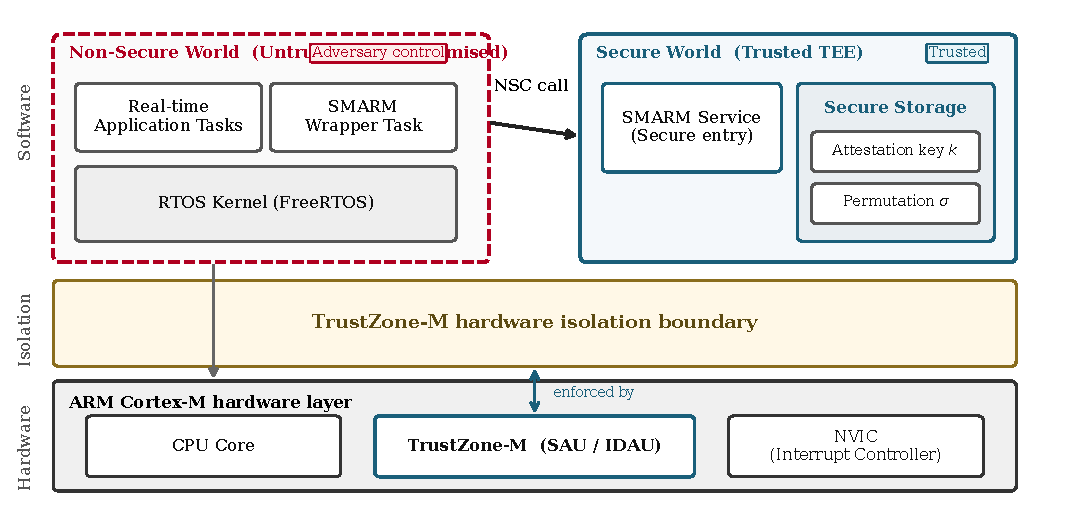
\includegraphics[width=1.0\linewidth]{system-threat-model.pdf}
  \caption{SMARM on FreeRTOS with TrustZone-M, as proposed in~\cite{smarmplus2026}.}
  \label{fig:system_model}
\end{figure}


% ================================================================
\section{Design}
\label{sec:design}

\subsection{Motivation}
\label{sec:motivation}

In the SMARM baseline, interrupts must be disabled throughout the measurement of each memory block. Consequently, the non-interruptibility period (\tdis), during which real-time tasks cannot execute, is determined by the time required to measure a single block. This duration depends primarily on two factors: the block size ($B$) and the measurement function.
%
% OLD:
% Following prior work~\cite{smarmplus2026,carpent2018smarm}, we investigated this issue using SHA-256 as the underlying measurement function. On an STM32 Nucleo-144 board, we observe that \tdis increases with $B$, from $0.062$~ms at $B{=}64$~bytes to $3.75$~ms at $B{=}4096$~bytes. For comparison, a high-frequency real-time task running at $1000$~Hz has a period of only 1~ms. Thus, with $B{=}4096$~bytes, a single SMARM block measurement can
% span several task periods and cause the real-time task to miss multiple
% deadlines. This makes the baseline SMARM unsuitable for such
% time-sensitive workloads.
\ben{Following prior work~\cite{smarmplus2026,carpent2018smarm}, we use a \emph{software} HMAC-SHA-256 implementation in the Secure world as the measurement function (no hardware crypto accelerator). On our Nucleo-144 board, baseline \tdis{} increases with $B$, from $0.060$~ms at $B{=}64$~bytes to $3.73$~ms at $B{=}4096$~bytes (DWT; Sec.~\ref{sec:eval}). For comparison, a $1000$~Hz real-time task has a period of only 1~ms. Thus, with $B{=}4096$~bytes, a single SMARM block measurement can span several task periods and cause the real-time task to miss multiple deadlines.}

% OLD:
% In this work, we observe that \tdis can be reduced without compromising SMARM's functionality or security guarantees.
\ben{In this work, we observe that \tdis{} can be reduced while preserving the temporal-consistency requirement of each block measurement.}
We notice that the security of each block measurement (in \textbf{[S1]}) inherently requires a \emph{temporal consistency} property~\cite{carpent2018temporal} in which the measurement result must faithfully correspond to a consistent state of the measured block at some point during the measurement.
The SMARM baseline achieves this property by measuring each block atomically with interrupts disabled, thereby preventing untrusted software from modifying the block while its contents are being hashed.

\emph{However, disabling interrupts throughout the entire measurement is not the only way to fulfill this property.}
The key requirement is instead to ensure a consistent \emph{capture} of the block contents that serve as input to the hash. Based on this observation, we propose two alternative mechanisms, \smarmcopy and \smarmlock, that preserve such consistency while substantially shortening the non-interruptibility period and allowing the hash computation itself to remain interruptible. Figure~\ref{fig:timing_diagram} compares their non-interruptibility periods with those of traditional RA and the SMARM baseline.

\begin{figure}[htbp]
  \centering
  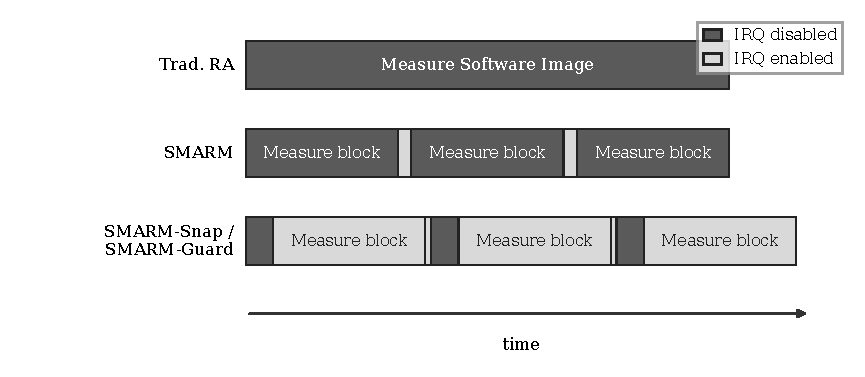
\includegraphics[width=1\linewidth]{timing_diagram.pdf}
  \caption{Comparison of non-interruptibility period between traditional RA, SMARM and our work}
  \label{fig:timing_diagram}
 
\end{figure}

\subsection{System and Threat Model}
\label{sec:system_threat}
We follow the system and threat models of prior work~\cite{smarmplus2026}. The prover is a resource-constrained IoT device equipped with a TrustZone-M TEE. 
It runs a commodity RTOS and application tasks in the Non-Secure world, while a small Trusted Computing Base (TCB), including the attestation service and its security-critical state, resides in the Secure world. 
The remote verifier is trusted and aims to determine the integrity of the prover's software while minimizing interference with real-time tasks scheduled to run intermittently on the prover.

We consider a software-level adversary (i.e., malware) with full control over the Non-Secure world, including the RTOS and applications. In particular, the adversary may employ \emph{roving malware} that relocates its malicious code during an ongoing attestation in an attempt to evade measurement. The Secure world and its TCB are trusted; thus, the adversary cannot compromise or modify code, data, or secrets residing in Secure memory.
We consider hardware attacks, including attacks that directly manipulate the hardware-enforced security attribution provided by the SAU/IDAU, to be out of scope. 



\begin{figure*}[t]
  \centering
  \raisebox{-10pt}{
\includegraphics[width=\textwidth]{combined_workflow.pdf}}  \caption{Shared SMARM loop (left) with three per-block measurement
    options (right). Red dashed regions mark interrupt-disabled steps.
    Baseline SMARM hashes under interrupts disabled; \smarmcopy{} copies
    under interrupts disabled then hashes with interrupts enabled;
    \smarmlock{} makes the selected block unavailable to Non-Secure
    software via the SAU, hashes in place with interrupts enabled, then
    restores Non-Secure availability.}
  \label{fig:combined_workflow}
\end{figure*}




\subsection{\smarmcopy}
\label{sec:atomic}

Our first enhancement achieves temporal consistency by taking an atomic snapshot of the shuffled memory block to be measured ($M_{\sigma[i]}$) and storing the snapshot in Secure-world RAM, where it is inaccessible to untrusted Non-Secure software. The subsequent measurement is then performed over this protected copy. We refer to this enhancement as \smarmcopy.

As illustrated in Fig.~\ref{fig:combined_workflow}, \smarmcopy follows the same overall workflow as the SMARM baseline and differs only in the per-block measurement operation. Rather than disabling interrupts for the entire measurement of $M_{\sigma[i]}$, \smarmcopy disables interrupts only while copying $M_{\sigma[i]}$ into Secure-world RAM.
Since the copy is performed atomically, the resulting snapshot corresponds to a consistent state of $M_{\sigma[i]}$.
Once the snapshot is complete, interrupts can be re-enabled and the measurement function can operate on the protected copy without interference from untrusted software.

The direct benefit of \smarmcopy is that it substantially shortens \tdis, since \tdis is reduced from the time required to hash a block to the time required only to copy it. On our Cortex-M33 target, the memory-copy throughput is around $17$~MB/s, giving
$t_{\mathrm{disabled}}^{\mathrm{copy}}\approx B/(17~\mathrm{MB/s})$, which is about $15\times$ shorter than the corresponding \tdis of the SMARM baseline.
%
The main drawback of \smarmcopy is that it requires a Secure-world storage of size 
$B$ to hold the snapshot. Our second enhancement, presented next, eliminates this additional storage cost.



\subsection{\smarmlock}
\label{sec:sau}

While \smarmcopy achieves temporal consistency by copying each block into a Secure-world buffer, this requires an additional $B$ bytes of Secure RAM. Our second enhancement, \smarmlock, avoids this storage overhead by making the memory block being measured, $M_{\sigma[i]}$, \emph{ephemerally inaccessible} to untrusted software.
This allows the SMARM service to measure the block \emph{in place} while interrupts remain enabled.

In our target system, we leverage the SAU to realize this mechanism. As shown in Figure~\ref{fig:combined_workflow}, before measuring $M_{\sigma[i]}$, \smarmlock reconfigures the SAU regions covering the attested memory so that $M_{\sigma[i]}$ is excluded from Non-Secure coverage.
%The SAU configurations before and during block measurement are shown in Figure~\ref{fig:sau_memory_map}. 
Since memory not explicitly attributed as Non-Secure is considered to be Secure by default in TrustZone-M, this effectively makes $M_{\sigma[i]}$ accessible only from the Secure world. 
The SAU update is followed by data and instruction synchronization barriers (\texttt{DSB} and \texttt{ISB}) to ensure that the new memory-security attribution takes effect immediately.

To preserve temporal consistency, the SAU reconfiguration and the associated barriers must execute atomically with interrupts disabled. However, this atomic operation is substantially shorter than either hashing or copying the entire block.
% OLD:
% In our measurements, each SAU attribution update takes only
% $0.80$-$1.30\,\mu$s ($87$-$143$ cycles at $110$~MHz).
\ben{Each block step comprises \emph{two} IRQ-off windows (lock, then unlock after the hash). In our DWT measurements, the mean duration of \emph{one} lock or unlock window is about $0.39$--$0.65\,\mu$s across $B$, with a worst-case single window of about $1.08\,\mu$s at large~$B$ (Sec.~\ref{sec:eval}); the sum of lock{+}unlock per block is about $0.8$--$1.3\,\mu$s.}
Once the block has been guarded, interrupts are re-enabled and the SMARM service measures $M_{\sigma[i]}$ directly. During this period, Non-Secure software may continue executing but cannot access $M_{\sigma[i]}$.

After the measurement completes, the SMARM service briefly disables interrupts to restore the original SAU configuration, making $M_{\sigma[i]}$ Non-Secure once again, and then proceeds to the next shuffled block $M_{\sigma[i+1]}$.
Thus, \smarmlock reduces each non-interruptibility period to a short SAU reconfiguration operation while keeping the substantially longer measurement computation interruptible. Unlike \smarmcopy, it requires no additional Secure-world storage.


\ignore{
\begin{figure}[!t]
  \centering
  \includegraphics[width=.8\linewidth]{sau_memory_map_compact.png}
  \caption{Non-Secure attribution of the attested flash before and
   during measurement. At rest, $|M|$ is fully Non-Secure; while
    $M_{\sigma(i)}$ is measured, two dynamic SAU regions leave the
    $B$-byte block uncovered (Secure by default). Interrupts are off
    only while the SAU is reprogrammed.}
  \label{fig:sau_memory_map}
\end{figure}
}


\ignore{
\begin{algorithm}[!ht]
\caption{\smarmlock{} Secure Service (TrustZone-M SAU instantiation)}
\label{alg:sau}
\begin{algorithmic}[1]
\Require $n$ blocks, shuffled indices $\sigma$, data window $M$, key $k$
\State \Call{HMAC.Init}{$k$}
\State \Call{SAU.RestoreWindowNS}{$M$} \Comment{rest state: $|M|$ is NS}
\For{$i \gets 0$ to $n-1$}
  \State $\mathit{blk} \gets M[\sigma(i)\cdot B]$
  \State \Call{DisableInterrupts}{}
  \State \Call{SAU.LockBlock}{\textit{blk}, $B$} \Comment{R6/R7; blk Secure-by-default}
  \State \Call{DSB}{}; \Call{ISB}{}
  \State \Call{EnableInterrupts}{}
  \State \Call{HMAC.Update}{\textit{blk}, $B$} \Comment{in place; interrupts on}
  \State \Call{DisableInterrupts}{}
  \State \Call{SAU.RestoreWindowNS}{$M$}
  \State \Call{DSB}{}; \Call{ISB}{}
  \State \Call{EnableInterrupts}{}
\EndFor
\State \textbf{return} \Call{HMAC.Finalize}{}
\end{algorithmic}
\end{algorithm}
}



\subsection{Security Guarantees}
\label{sec:security_summary}

% OLD:
% Both \smarmcopy and \smarmlock modify only how each shuffled memory block is measured; they do not alter the underlying SMARM protocol. In particular, the attestation key $k$ and secret permutation $\sigma$ are generated, used, and stored exactly as in the SMARM baseline. Therefore, \textbf{[S2] Key Secrecy} and \textbf{[S3] Private Measurement Order} continue to hold. 
% Likewise, both designs preserve SMARM's controlled execution interface, where the attestation functionality remains within the Secure-world SMARM Service and can be invoked from the Non-Secure world only through its designated NSC entry point.
% The main change concerns \textbf{[S1] Controlled Execution}. ...
% Thus, \smarmcopy and \smarmlock preserve \textbf{[S1]} through two different mechanisms.
% As such, with the unchanged guarantees of \textbf{[S2]} and \textbf{[S3]}, both enhancements retain the security guarantees of the SMARM baseline.

\ben{Both designs change only how each shuffled block is captured; the SMARM protocol, key~$k$, and permutation~$\sigma$ remain in Secure world and are reachable from Non-Secure world only via the designated NSC entry.
\textbf{[S1]} is preserved: \smarmcopy{} captures an atomic Secure snapshot before hashing with interrupts enabled, while \smarmlock{} makes $M_{\sigma[i]}$ inaccessible to Non-Secure software during the in-place hash.
\textbf{[S2]} is unchanged: $k$ remains in Secure memory.
The permutation~$\sigma$ also remains in Secure memory for both designs.
\smarmcopy{} introduces no new observable signal about the current block, because hashing uses a Secure snapshot.
For \smarmlock{}, however, concurrent Non-Secure accesses to a guarded block may exhibit distinguishable access or timing behavior and thereby reveal information about the current measurement block.
We therefore do not claim baseline-equivalent order privacy for \smarmlock{} under active probing.
Our evaluation uses a dedicated Non-Secure data window (Sec.~\ref{sec:eval}); when continuous Non-Secure access is required during measurement, \smarmcopy{} or baseline SMARM is preferable.
Quantifying this leakage is left to future work.}


\section{Evaluation}
\label{sec:eval}

\subsection{Setup}

% OLD:
% We evaluate \smarmcopy and \smarmlock on an STM32 Nucleo-144 development board equipped with a Cortex-M33 MCU and TrustZone-M. The MCU runs at $110$~MHz and executes FreeRTOS and real-time applications in the Non-Secure world. 
% We configure $512$~KiB of the entire Non-Secure flash as the attested memory region, yielding the total attested memory size of $|M|{=}512$~KiB.
% We evaluate all three designs across six block sizes,
% $B\in\{128,256,512,1024,2048,4096\}$~bytes; we use the following evaluation metrics: the non-interruptibility period (\tdis), secure memory overhead, real-time availability, and an end-to-end attestation runtime.
\ben{We evaluate the SMARM baseline, \smarmcopy, and \smarmlock on an STM32 Nucleo-144 (STM32L552ZE, TrustZone-M) at $110$~MHz with FreeRTOS in the Non-Secure world. The MCU has $512$~KiB flash in total, split into Secure and Non-Secure banks of $256$~KiB each. For a fair same-harness comparison we attest a fixed dedicated Non-Secure data window $|M|{=}128$~KiB with one shuffled pass. Measurement uses software HMAC-SHA-256 in Secure world (no hardware crypto accelerator). We evaluate $B\in\{64,128,256,512,1024,2048,4096\}$~bytes and report \tdis, Secure RAM, measured FAR at $1000$~Hz, and end-to-end runtime.}

\subsection{Non-interruptibility Period}

% OLD:
% Figure~\ref{fig:tdisabled} compares \tdis{} of the SMARM baseline, \smarmcopy, and \smarmlock{} on a logarithmic scale. Across all three designs, \tdis{} increases with the block size $B$, as larger blocks require more work during the corresponding uninterruptible operation.
%
% Compared with the baseline, \smarmcopy{} reduces \tdis{} by approximately one order of magnitude (about $15\times$) by replacing the per-block hash within the interrupt-disabled period with a substantially faster memory copy. At $B{=}4096$~bytes, \tdis{} decreases from $3.75$~ms in the baseline to about $0.24$~ms with \smarmcopy.
%
% \smarmlock{} further reduces \tdis{} by limiting interrupt disablement to the short SAU reconfiguration operations required to protect and restore each block. At $B{=}4096$~bytes, \tdis{} is around $0.8$-$1.3\,\mu$s, corresponding to a reduction of roughly three orders of magnitude compared with the baseline.
%
% Overall, these results show that \smarmcopy{} and \smarmlock{} substantially shorten SMARM's non-interruptibility period, reducing it from the millisecond range in the baseline to the sub-millisecond and microsecond ranges, respectively.

\paragraph{\ben{Measurement method.}}
\ben{We enable the Cortex-M DWT cycle counter in Secure world and record $\mathrm{CYCCNT}$ immediately inside each \texttt{\_\_disable\_irq}/\texttt{\_\_enable\_irq} window ($110$~MHz $\Rightarrow$ $1$~cycle $=1/110\,\mu$s). For baseline SMARM the window is one HMAC-update of size~$B$; for \smarmcopy{} it is the \texttt{memcpy} of size~$B$; for \smarmlock{} each lock and each unlock is a separate window. We report the \emph{mean} over all windows in a round (ten rounds); for schedulability the \emph{worst-case} single window also matters (e.g., Guard max $\approx 1.08\,\mu$s at $B{=}4096$).}

\ben{Figure~\ref{fig:tdisabled} and Table~\ref{tab:tdisabled} summarize the results. Baseline and \smarmcopy{} \tdis{} grow roughly linearly with~$B$ (hash or copy work). \smarmlock{} remains nearly independent of~$B$, staying in the sub-microsecond to $\sim\!\!1\,\mu$s range; the small observed variation across~$B$ reflects measurement-level variability rather than block-size-dependent hashing, which occurs with interrupts enabled. At $B{=}4096$, mean \tdis{} falls from $3.73$~ms (baseline) to $0.243$~ms (\smarmcopy{}, $\sim\!\!15\times$) and to $0.65\,\mu$s mean / $1.08\,\mu$s max (\smarmlock{}, roughly three to four orders of magnitude).}


\begin{figure}[ht]
  \centering
  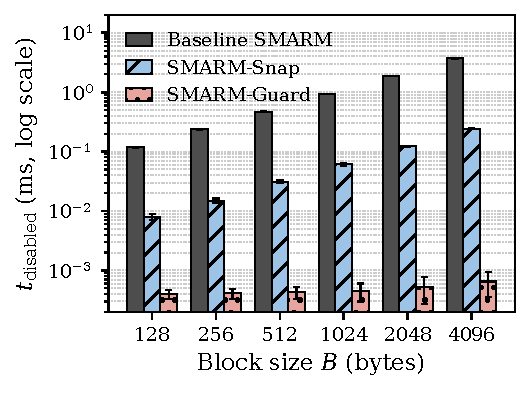
\includegraphics[width=.95\linewidth]{tdisabled_three_log_1.pdf}
  \caption{\ben{Non-interruptibility period (\tdis) across designs (log $y$-axis). Guard bars are mean per lock/unlock window (DWT @ $110$~MHz).}}
  % OLD: Non-interruptibility period (\tdis) across different designs; y-axis is displayed in a log scale.
  \label{fig:tdisabled}
\end{figure}

% NEW table (M5):
\begin{table}[ht]
  \centering
  \caption{\ben{Mean \tdis{} (DWT): Baseline/\smarmcopy{} in ms; \smarmlock{} mean window in $\mu$s.}}
  \label{tab:tdisabled}
  \small
  \setlength{\tabcolsep}{3.5pt}
  \begin{tabularx}{\columnwidth}{@{}lXXXXXXX@{}}
    \toprule
    \textbf{$B$} & 64 & 128 & 256 & 512 & 1024 & 2048 & 4096 \\
    \midrule
    Baseline (ms) & 0.060 & 0.119 & 0.235 & 0.469 & 0.935 & 1.867 & 3.731 \\
    \smarmcopy{} (ms) & 0.001 & 0.008 & 0.015 & 0.031 & 0.061 & 0.122 & 0.243 \\
    \smarmlock{} ($\mu$s) & 0.39 & 0.40 & 0.41 & 0.42 & 0.45 & 0.52 & 0.65 \\
    \bottomrule
  \end{tabularx}
\end{table}

\subsection{Secure Memory Overhead}

\smarmcopy{} requires an additional Secure buffer of size~$B$ for the snapshot. \smarmlock{} introduces no additional Secure RAM beyond the SMARM baseline.


\subsection{Real-Time Availability}

% OLD:
% We evaluate real-time availability using the Frequency Accuracy Ratio (FAR) metric proposed in~\cite{smarmplus2026}, defined as:
% \begin{align*}
%     \mathrm{FAR} = f_{\mathrm{observed}} / f_{\mathrm{baseline}}
% \end{align*}
% where $f_{\mathrm{observed}}$ is the observed execution frequency of a periodic real-time task while attestation is active, and $f_{\mathrm{baseline}}$ is its execution frequency under the same attestation workload but without interrupt disablement. Thus, $\mathrm{FAR}\approx1.0$ indicates that attestation introduces little interference with the execution frequency of the real-time task, whereas a lower FAR indicates increasing interference.
%
% As shown in~\cite{smarmplus2026}, under a $1000$~Hz real-time workload, the FAR of the SMARM baseline decreases significantly as $B$ increases, particularly when \tdis becomes longer than the task period. 
% In contrast, both \smarmcopy{} and \smarmlock{} maintain $\mathrm{FAR}\approx1.0$ across all evaluated block sizes, including $B{=}4096$~bytes. These results show that the substantial reductions in \tdis{} achieved by our enhancements translate directly into improved real-time availability, allowing high-frequency real-time tasks to continue executing with negligible interference during attestation.

\ben{We evaluate real-time availability using the Frequency Accuracy Ratio $\mathrm{FAR}=f_{\mathrm{observed}}/f_{\mathrm{baseline}}$~\cite{smarmplus2026}, where $f_{\mathrm{observed}}$ is the activation frequency of a periodic FreeRTOS task (\texttt{osDelayUntil}, $1000$~Hz, higher priority than the attestation wrapper) during an attestation round, and $f_{\mathrm{baseline}}$ is the nominal $1000$~Hz rate. Table~\ref{tab:far} reports mean FAR over ten rounds on the same $|M|{=}128$~KiB harness. Baseline SMARM maintains $\mathrm{FAR}=1.000$ for $B\leq 1024$, where the IRQ-off window remains below the $1$~ms tick, but drops to $0.54$ and $0.27$ at $B{=}2048$ and $4096$, respectively, consistent with lost SysTick releases when the interrupt-disabled window exceeds one tick. Both \smarmcopy{} and \smarmlock{} keep $\mathrm{FAR}=1.000$ for every tested~$B$, including $4096$.}

% NEW (M4):
\begin{table}[ht]
  \centering
  \caption{\ben{Measured FAR at $1000$~Hz ($|M|{=}128$~KiB, ten rounds).}}
  \label{tab:far}
  \small
  \setlength{\tabcolsep}{3.5pt}
  \begin{tabularx}{\columnwidth}{@{}lXXXXXXX@{}}
    \toprule
    \textbf{$B$} & 64 & 128 & 256 & 512 & 1024 & 2048 & 4096 \\
    \midrule
    Baseline & 1.00 & 1.00 & 1.00 & 1.00 & 1.00 & 0.54 & 0.27 \\
    \smarmcopy & 1.00 & 1.00 & 1.00 & 1.00 & 1.00 & 1.00 & 1.00 \\
    \smarmlock & 1.00 & 1.00 & 1.00 & 1.00 & 1.00 & 1.00 & 1.00 \\
    \bottomrule
  \end{tabularx}
\end{table}


\subsection{Attestation Runtime}

% OLD:
% Reducing \tdis does not necessarily shorten the end-to-end attestation runtime, since computing the MAC over the entire attested memory region, $|M|{=}512$~KiB, still dominates the overall cost. Table~\ref{tab:attest_runtime} reports the mean end-to-end attestation runtime of the three designs across different block sizes.
%
% Across all evaluated block sizes, the baseline SMARM and \smarmlock exhibit comparable runtimes, ranging from approximately $480$~ms at $B{=}4096$~bytes to about $560$~ms at $B{=}128$~bytes. In contrast, \smarmcopy is consistently around $30$~ms slower than the other two designs. This additional overhead results from the extra memory-copy operation required to capture each block into Secure-world RAM before it is measured.
%
% Overall, these results show that the substantial reduction in \tdis achieved by our enhancements does not come at the cost of a significant increase in total attestation runtime: \smarmlock incurs essentially no additional end-to-end overhead, while \smarmcopy introduces only a modest overhead due to block copying.
%
% \begin{table}[t]
%   \centering
%   \caption{End-to-end attestation time (ms) for $|M|=512$~KiB without concurrent real-time task (ten rounds; SD~$<1$~ms).}
%   \label{tab:attest_runtime}
%   \footnotesize
%   \setlength{\tabcolsep}{3.5pt}
%   \begin{tabularx}{\columnwidth}{@{}lXXXXXXX@{}}
%     \toprule
%     \textbf{$B$ (bytes)} & 128 & 256 & 512 & 1024 & 2048 & 4096 \\
%     \midrule
%     Baseline SMARM & 567 & 521 & 500 & 490 & 484 & 481 \\
%     \smarmcopy & 592 & 550 & 529 & 519 & 513 & 511 \\
%     \smarmlock & 559 & 517 & 497 & 487 & 482 & 480 \\
%     \bottomrule
%   \end{tabularx}
% \end{table}

\ben{Reducing \tdis{} does not proportionally shorten end-to-end runtime: HMAC over $|M|{=}128$~KiB still dominates (Table~\ref{tab:attest_runtime}; ten rounds, no concurrent RT task, SD~$<1$~ms). Baseline and \smarmlock{} differ by only a few milliseconds across~$B$; we do \emph{not} claim that \smarmlock{} is faster. Each Guard block adds lock{+}unlock of about $0.8$--$1.3\,\mu$s, i.e., about $1.6$--$2.7$~ms aggregate at $B{=}64$ ($2048$ blocks), which cannot explain larger gaps, and remaining differences are not interpreted as a systematic speedup because the experiment does not isolate harness-level timing effects. \smarmcopy{} adds about $7$--$8$~ms on this harness due to copying.}

\begin{table}[ht]
  \centering
  \caption{\ben{End-to-end attestation time (ms), $|M|{=}128$~KiB, ten rounds, no RT task (SD~$<1$~ms).}}
  \label{tab:attest_runtime}
  \small
  \setlength{\tabcolsep}{3.5pt}
  \begin{tabularx}{\columnwidth}{@{}lXXXXXXX@{}}
    \toprule
    \textbf{$B$ (bytes)} & 64 & 128 & 256 & 512 & 1024 & 2048 & 4096 \\
    \midrule
    Baseline SMARM & 164 & 142 & 131 & 125 & 123 & 121 & 120 \\
    \smarmcopy & 165 & 149 & 138 & 132 & 130 & 128 & 128 \\
    \smarmlock & 159 & 140 & 130 & 125 & 122 & 121 & 121 \\
    \bottomrule
  \end{tabularx}
\end{table}


\subsection{Summary}
\label{sec:guidance}

% [H] keeps Table IV in source order (before Conclusion/References); [t] was deferred past the bibliography.
\begin{table}[H]
  \centering
  \caption{\ben{Comparison of attestation approaches (TrustZone-M / FreeRTOS).}}
  \label{tab:ra_comparison}
  \renewcommand{\arraystretch}{1.08}
  \small
  \setlength{\tabcolsep}{4pt}
  \begin{tabularx}{\columnwidth}{@{}
      >{\raggedright\arraybackslash}X
      c c c@{}}
    \toprule
    \textbf{Approach} &
    \makecell{\textbf{FAR$\,{\approx}\,1$} \\ \textbf{@1000~Hz}} &
    \makecell{\textbf{Extra} \\ \textbf{Secure RAM}} &
    \makecell{\textbf{\tdis} \\ \textbf{scale}} \\
    \midrule
    Traditional RA~\cite{eldefrawy2012smart,eldefrawy2017hydra,nunes2019vrased} &
    \texttimes & 0 & $\sim\!10^{2}$--$10^{3}$~ms \\
    SMARM (TZ-M baseline)~\cite{smarmplus2026} &
    Partial & 0 & $\sim\!10^{-1}$--$10^{0}$~ms \\
    \textbf{\smarmcopy} &
    \checkmark & $B$ & $\sim\!10^{-3}$--$10^{-1}$~ms \\
    \textbf{\smarmlock} &
    \checkmark & 0 & $\sim\!\mu$s \\
    \bottomrule
  \end{tabularx}
\end{table}

\ben{Table~\ref{tab:ra_comparison} summarizes the trade-off: \smarmcopy{} needs a Secure buffer of size~$B$, while \smarmlock{} needs none and is evaluated on a dedicated Non-Secure data window; if continuous Non-Secure access is required during measurement, prefer \smarmcopy{} or baseline SMARM.}

\section{Conclusion}
\label{sec:conclusion}
\ben{SMARM allows interrupts between memory blocks, but per-block hashing can still stall high-frequency real-time tasks when blocks are large. We propose two complementary FreeRTOS/TrustZone-M enhancements. \smarmcopy{} shortens the non-interruptibility period to a brief Secure-world memory copy at the cost of a Secure buffer of size~$B$. \smarmlock{} instead uses a brief SAU update with no extra buffer, under a dedicated Non-Secure data-window assumption. On our platform, \smarmcopy{} reduces \tdis{} by about one order of magnitude ($\sim\!\!15\times$) and \smarmlock{} by roughly three to four orders at large~$B$; both keep measured FAR~$=1.0$ at $1000$~Hz in the evaluated harness. \smarmlock{} does not claim baseline-equivalent order privacy under concurrent active probing (Sec.~\ref{sec:security_summary}).}


% SMARM improves RA interactivity by allowing interrupts between blocks,
% but its per-block interrupt-disabled hash still yields a long
% \tdis{} for large~$B$ on FreeRTOS/TrustZone-M.
% \smarmcopy{} shortens that window to a Secure-world memory copy
% and restores FAR~$\approx 1.0$ under a $1000$~Hz workload, at the cost
% of a Secure buffer of size~$B$.
% \smarmlock{} achieves a still shorter \tdis{} without that buffer by
% making each measured block ephemerally unavailable to Non-Secure
% software via brief SAU updates, then hashing in place with interrupts
% enabled; it likewise maintains FAR~$\approx 1.0$ at $1000$~Hz across
% the evaluated block sizes.
% Both enhancements preserve SMARM's security properties~(S1)--(S3):
% controlled Secure/NSC entry with integrity of each block capture,
% secrecy of~$k$, and privacy of the measurement order~$\sigma$.
% In practice, prefer \smarmcopy{} when Secure RAM of size~$B$ is
% available or the SAU must remain fixed after boot, and prefer
% \smarmlock{} when a dedicated Non-Secure data window~$|M|$ can absorb
% brief SAU attribution changes without an extra Secure buffer.

{\footnotesize
\bibliographystyle{IEEEtran}
\bibliography{citation}
}

\end{document}
